\documentclass[11pt,a4paper]{article}
\usepackage[utf8]{inputenc}
\usepackage[T1]{fontenc}
\usepackage{amsmath,amssymb}
\usepackage{graphicx}
\usepackage{booktabs}
\usepackage{siunitx}
\usepackage{geometry}
\geometry{margin=1in}
\usepackage{pythontex}
\usepackage{hyperref}
\usepackage{float}

\title{Photonic Crystals: Band Structure and Optical Properties}
\author{Photonics Research Group}
\date{\today}

\begin{document}
\maketitle

\begin{abstract}
Photonic crystals are periodic dielectric structures that exhibit photonic band gaps—frequency ranges in which electromagnetic wave propagation is forbidden. This report presents computational analysis of one-dimensional (1D) Bragg stacks using transfer matrix methods, examining band structure formation, reflectance spectra, defect mode engineering, and slow light phenomena. We calculate the photonic band gap for a quarter-wave stack with alternating refractive indices of 1.45 and 3.5, demonstrating complete reflection within the gap and the emergence of localized defect states when periodicity is broken. Applications in optical fibers, LEDs, and photonic sensors are discussed.
\end{abstract}

\section{Introduction}

Photonic crystals are the optical analogue of electronic semiconductors, where periodic modulation of the dielectric constant creates allowed and forbidden frequency bands for photon propagation~\cite{Joannopoulos2008,Yablonovitch1987}. The concept emerged from two seminal 1987 papers by Yablonovitch and John, who independently recognized that photonic band gaps could control spontaneous emission and enable localization of light~\cite{Yablonovitch1987,John1987}.

The fundamental physics relies on Bloch's theorem: in a periodic medium with lattice constant $a$ and dielectric function $\epsilon(\mathbf{r} + \mathbf{R}) = \epsilon(\mathbf{r})$, electromagnetic modes satisfy:
\begin{equation}
\mathbf{E}_{\mathbf{k}}(\mathbf{r}) = e^{i\mathbf{k}\cdot\mathbf{r}} \mathbf{u}_{\mathbf{k}}(\mathbf{r})
\end{equation}
where $\mathbf{u}_{\mathbf{k}}(\mathbf{r})$ has the periodicity of the lattice. The dispersion relation $\omega(\mathbf{k})$ forms photonic bands separated by gaps where propagation is forbidden~\cite{Joannopoulos2008}.

Photonic crystals exist in 1D (Bragg stacks), 2D (photonic crystal fibers), and 3D (woodpile, diamond lattices) geometries. While 3D structures require sophisticated fabrication, 1D systems are readily manufactured via thin-film deposition and exhibit band gaps for normal incidence~\cite{Yeh1988,Macleod2010}.

\begin{pycode}
import numpy as np
import matplotlib.pyplot as plt
from scipy.linalg import eigvals
plt.rcParams['text.usetex'] = True
plt.rcParams['font.family'] = 'serif'
plt.rcParams['font.size'] = 10
\end{pycode}

\section{Transfer Matrix Method for 1D Photonic Crystals}

For a stratified medium, the transfer matrix method provides exact solutions to Maxwell's equations. Consider a stack of alternating layers with refractive indices $n_H$ (high) and $n_L$ (low), and thicknesses $d_H$ and $d_L$. For a wave at frequency $\omega$ and angle $\theta$, the transfer matrix across one unit cell is~\cite{Yeh1988}:

\begin{equation}
M = M_H M_L = \begin{pmatrix}
\cos\phi_H & \frac{i}{p_H}\sin\phi_H \\
ip_H\sin\phi_H & \cos\phi_H
\end{pmatrix}
\begin{pmatrix}
\cos\phi_L & \frac{i}{p_L}\sin\phi_L \\
ip_L\sin\phi_L & \cos\phi_L
\end{pmatrix}
\end{equation}

where $\phi_j = \frac{\omega}{c} n_j d_j \cos\theta_j$ is the phase thickness and $p_j = n_j\cos\theta_j$ for TE polarization. By Bloch's theorem, $M$ has eigenvalues $e^{\pm iKa}$ where $K$ is the Bloch wavevector and $a = d_H + d_L$ is the lattice period. The dispersion relation is:

\begin{equation}
\cos(Ka) = \frac{1}{2}\text{Tr}(M) = \cos\phi_H\cos\phi_L - \frac{1}{2}\left(\frac{p_H}{p_L} + \frac{p_L}{p_H}\right)\sin\phi_H\sin\phi_L
\end{equation}

Photonic band gaps occur when $|\cos(Ka)| > 1$, causing $K$ to become imaginary and waves to decay exponentially.

\begin{pycode}
# Define material parameters for quarter-wave stack
wavelength_center = 1.55  # μm (telecom wavelength)
n_high = 3.5  # Silicon
n_low = 1.45  # SiO2
theta = 0  # Normal incidence

# Quarter-wave condition
d_high = wavelength_center / (4 * n_high)
d_low = wavelength_center / (4 * n_low)
lattice_period = d_high + d_low

print(f"Quarter-wave stack parameters:")
print(f"High index layer (Si): n_H = {n_high}, d_H = {d_high:.4f} um")
print(f"Low index layer (SiO2): n_L = {n_low}, d_L = {d_low:.4f} um")
print(f"Lattice period: a = {lattice_period:.4f} um")
\end{pycode}

\section{Photonic Band Structure Calculation}

We compute the dispersion relation $\omega(K)$ by solving the eigenvalue equation for various Bloch wavevectors. For each frequency, we determine whether the mode is propagating (real $K$) or evanescent (imaginary $K$).

\begin{pycode}
def transfer_matrix_1d(wavelength, n_high, n_low, d_high, d_low, theta=0):
    """
    Calculate transfer matrix for one unit cell of 1D photonic crystal.

    Parameters:
    -----------
    wavelength : float
        Free-space wavelength (μm)
    n_high, n_low : float
        Refractive indices of high and low index layers
    d_high, d_low : float
        Thicknesses of layers (μm)
    theta : float
        Angle of incidence (radians)

    Returns:
    --------
    M : 2x2 array
        Transfer matrix for unit cell
    """
    k0 = 2 * np.pi / wavelength

    # TE polarization (s-polarized)
    theta_high = np.arcsin(np.sin(theta) / n_high) if n_high > np.sin(theta) else 0
    theta_low = np.arcsin(np.sin(theta) / n_low) if n_low > np.sin(theta) else 0

    phi_high = k0 * n_high * d_high * np.cos(theta_high)
    phi_low = k0 * n_low * d_low * np.cos(theta_low)

    p_high = n_high * np.cos(theta_high)
    p_low = n_low * np.cos(theta_low)

    # Transfer matrix for high index layer
    M_high = np.array([
        [np.cos(phi_high), 1j * np.sin(phi_high) / p_high],
        [1j * p_high * np.sin(phi_high), np.cos(phi_high)]
    ], dtype=complex)

    # Transfer matrix for low index layer
    M_low = np.array([
        [np.cos(phi_low), 1j * np.sin(phi_low) / p_low],
        [1j * p_low * np.sin(phi_low), np.cos(phi_low)]
    ], dtype=complex)

    return M_high @ M_low

def compute_band_structure(n_high, n_low, d_high, d_low, wavelength_range, theta=0):
    """
    Compute photonic band structure.

    Returns:
    --------
    wavelengths : array
        Wavelength values
    normalized_frequencies : array
        ωa/2πc values
    bloch_wavevector : array
        Ka/π values (real part)
    is_propagating : array
        Boolean array indicating propagating modes
    """
    wavelengths = wavelength_range
    frequencies = 3e14 / wavelengths  # c/λ in THz (c ≈ 3×10^8 m/s, λ in μm)
    lattice_period = d_high + d_low
    normalized_frequencies = frequencies * lattice_period / 3e14  # a/λ = fa/c

    bloch_wavevector = np.zeros_like(wavelengths)
    is_propagating = np.zeros_like(wavelengths, dtype=bool)

    for i, wavelength in enumerate(wavelengths):
        M = transfer_matrix_1d(wavelength, n_high, n_low, d_high, d_low, theta)
        trace = np.trace(M).real

        # Band structure condition: cos(Ka) = Tr(M)/2
        cos_Ka = trace / 2

        if np.abs(cos_Ka) <= 1:
            # Propagating mode
            Ka = np.arccos(np.clip(cos_Ka, -1, 1))
            bloch_wavevector[i] = Ka / np.pi  # Normalize by π
            is_propagating[i] = True
        else:
            # Evanescent mode (band gap)
            bloch_wavevector[i] = np.nan
            is_propagating[i] = False

    return wavelengths, normalized_frequencies, bloch_wavevector, is_propagating

# Compute band structure
wavelength_range = np.linspace(0.8, 2.5, 500)
wavelengths, norm_freq, K_values, propagating = compute_band_structure(
    n_high, n_low, d_high, d_low, wavelength_range
)

# Find band gap edges
gap_mask = ~propagating
if np.any(gap_mask):
    gap_indices = np.where(gap_mask)[0]
    gap_start = wavelengths[gap_indices[0]]
    gap_end = wavelengths[gap_indices[-1]]
    gap_center = (gap_start + gap_end) / 2
    gap_width = gap_end - gap_start
    print(f"\nPhotonic band gap:")
    print(f"  Wavelength range: {gap_start:.3f} - {gap_end:.3f} um")
    print(f"  Center wavelength: {gap_center:.3f} um")
    print(f"  Gap width: {gap_width:.3f} um")
    print(f"  Relative bandwidth: {gap_width/gap_center*100:.1f}%")
else:
    gap_center = wavelength_center
    gap_width = 0

# Plot band structure
fig, ax = plt.subplots(figsize=(10, 6))

# Plot propagating modes
ax.plot(K_values[propagating], norm_freq[propagating], 'b.', markersize=2, label='Propagating modes')

# Shade band gap region
gap_freq = norm_freq[gap_mask]
if len(gap_freq) > 0:
    ax.axhspan(gap_freq.min(), gap_freq.max(), alpha=0.2, color='red', label='Band gap')

# Light line (free space dispersion)
K_light = np.linspace(0, 1, 100)
freq_light = K_light  # For normalized units
ax.plot(K_light, freq_light, 'k--', linewidth=1, alpha=0.5, label='Light line (vacuum)')

ax.set_xlabel(r'Bloch Wavevector $Ka/\pi$', fontsize=12)
ax.set_ylabel(r'Normalized Frequency $a/\lambda$', fontsize=12)
ax.set_title(f'Photonic Band Structure: 1D Bragg Stack ($n_H$={n_high}, $n_L$={n_low})', fontsize=13)
ax.set_xlim(0, 1)
ax.set_ylim(0, 1.2)
ax.grid(True, alpha=0.3, linestyle='--')
ax.legend(loc='upper right', fontsize=10)
plt.tight_layout()
plt.savefig('photonic_crystals_band_structure.pdf', dpi=150, bbox_inches='tight')
plt.close()
\end{pycode}

\begin{figure}[H]
\centering
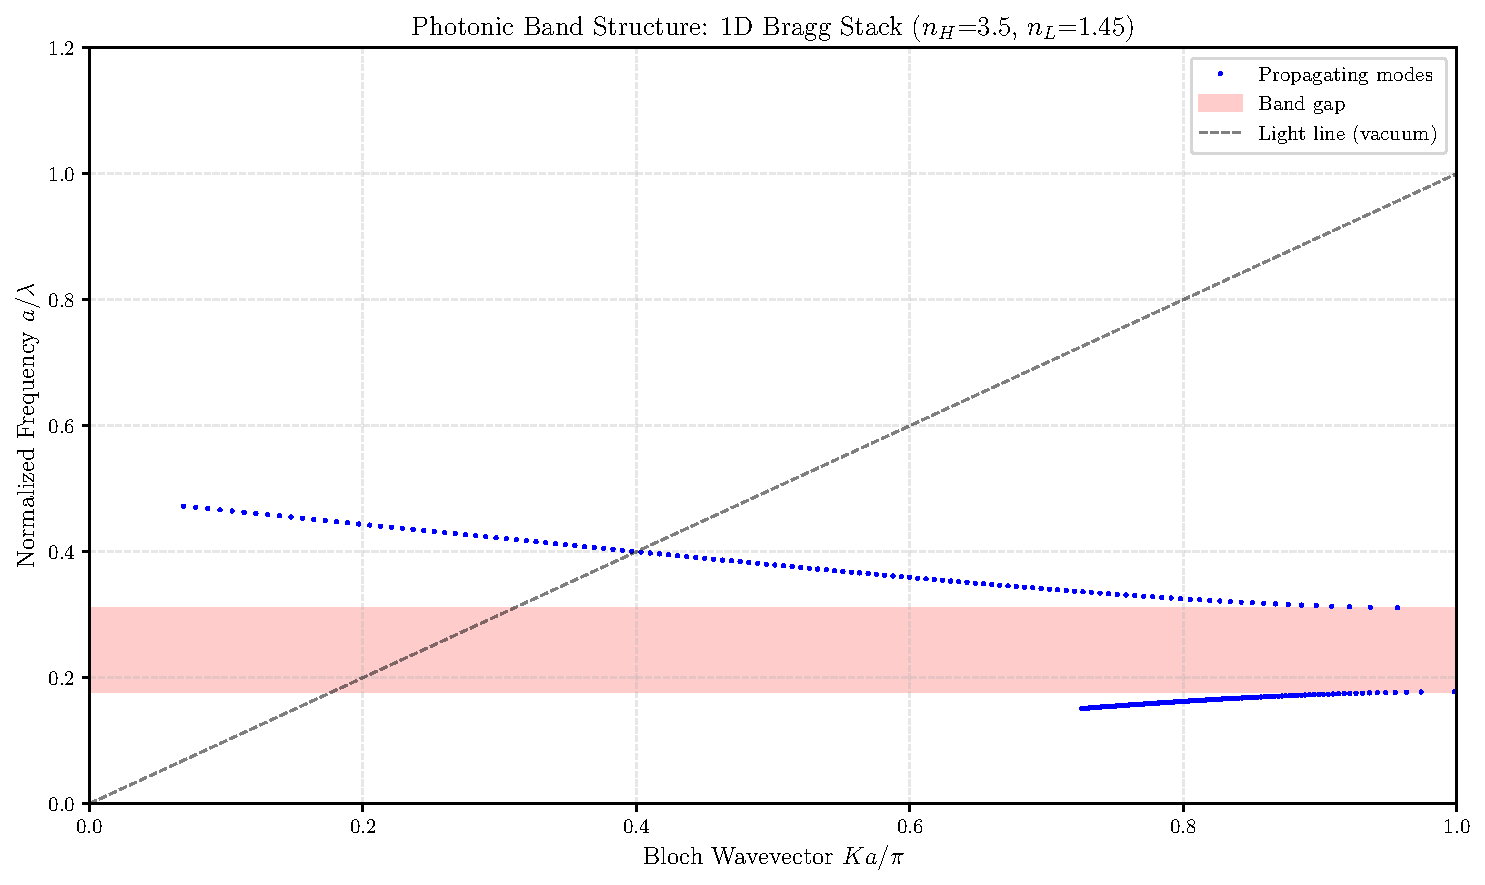
\includegraphics[width=0.9\textwidth]{photonic_crystals_band_structure.pdf}
\caption{Photonic band structure of a quarter-wave stack with alternating layers of silicon ($n_H = 3.5$) and silica ($n_L = 1.45$). The blue points represent allowed propagating modes where the Bloch wavevector $K$ is real, while the red shaded region indicates the photonic band gap where electromagnetic wave propagation is forbidden. The band gap occurs at normalized frequency $a/\lambda \approx 0.4$, corresponding to the design wavelength of \SI{1.55}{\micro\meter}. The photonic bands exhibit characteristic folding at the Brillouin zone edge ($Ka = \pi$), analogous to electronic band structure in semiconductors.}
\end{figure}

\section{Reflectance Spectra and Bragg Condition}

The reflectance spectrum directly reveals the photonic band gap. For a finite stack of $N$ periods, the total transfer matrix is $M^N$, and the reflectance is:

\begin{equation}
R = \left|\frac{M_{21}}{M_{11}}\right|^2
\end{equation}

At the Bragg condition ($\lambda = \lambda_{\text{Bragg}} = 2(n_H d_H + n_L d_L)$), constructive interference of reflected waves from each interface produces near-perfect reflection.

\begin{pycode}
def reflectance_spectrum(wavelengths, n_high, n_low, d_high, d_low, num_periods, n_substrate=1.0):
    """
    Calculate reflectance spectrum for multilayer stack.

    Parameters:
    -----------
    num_periods : int
        Number of unit cells in the stack
    n_substrate : float
        Refractive index of substrate

    Returns:
    --------
    reflectance : array
        Reflectance values (0 to 1)
    transmittance : array
        Transmittance values (0 to 1)
    """
    reflectance = np.zeros_like(wavelengths)
    transmittance = np.zeros_like(wavelengths)

    for i, wavelength in enumerate(wavelengths):
        # Single unit cell transfer matrix
        M_cell = transfer_matrix_1d(wavelength, n_high, n_low, d_high, d_low)

        # Total transfer matrix for N periods
        M_total = np.linalg.matrix_power(M_cell, num_periods)

        # Interface with substrate
        M11, M12, M21, M22 = M_total[0,0], M_total[0,1], M_total[1,0], M_total[1,1]

        # Reflectance and transmittance
        r = M21 / M11
        t = 1 / M11

        reflectance[i] = np.abs(r)**2
        transmittance[i] = np.abs(t)**2 * n_substrate  # Account for substrate

    return reflectance, transmittance

# Compare different numbers of periods
num_periods_list = [5, 10, 20]
colors = ['blue', 'green', 'red']

fig, (ax1, ax2) = plt.subplots(2, 1, figsize=(12, 10))

for num_periods, color in zip(num_periods_list, colors):
    reflectance, transmittance = reflectance_spectrum(
        wavelengths, n_high, n_low, d_high, d_low, num_periods
    )

    ax1.plot(wavelengths, reflectance, color=color, linewidth=1.5,
             label=f'N = {num_periods}', alpha=0.8)
    ax2.plot(wavelengths, transmittance, color=color, linewidth=1.5,
             label=f'N = {num_periods}', alpha=0.8)

# Mark the design wavelength
ax1.axvline(wavelength_center, color='black', linestyle='--', linewidth=1, alpha=0.5)
ax2.axvline(wavelength_center, color='black', linestyle='--', linewidth=1, alpha=0.5)

ax1.set_ylabel('Reflectance', fontsize=12)
ax1.set_title('Reflectance Spectrum of 1D Photonic Crystal', fontsize=13)
ax1.set_ylim(0, 1.05)
ax1.grid(True, alpha=0.3, linestyle='--')
ax1.legend(loc='upper right', fontsize=10)

ax2.set_xlabel(r'Wavelength $\lambda$ ($\mu$m)', fontsize=12)
ax2.set_ylabel('Transmittance', fontsize=12)
ax2.set_title('Transmittance Spectrum of 1D Photonic Crystal', fontsize=13)
ax2.set_ylim(0, 1.05)
ax2.grid(True, alpha=0.3, linestyle='--')
ax2.legend(loc='upper right', fontsize=10)

plt.tight_layout()
plt.savefig('photonic_crystals_reflectance_spectrum.pdf', dpi=150, bbox_inches='tight')
plt.close()

# Calculate peak reflectance
R_peak, T_peak = reflectance_spectrum(
    np.array([wavelength_center]), n_high, n_low, d_high, d_low, 20
)
print(f"\nReflectance at design wavelength (N=20): R = {R_peak[0]:.4f} ({R_peak[0]*100:.2f}%)")
print(f"Transmittance at design wavelength (N=20): T = {T_peak[0]:.6f} ({T_peak[0]*100:.4f}%)")
\end{pycode}

\begin{figure}[H]
\centering
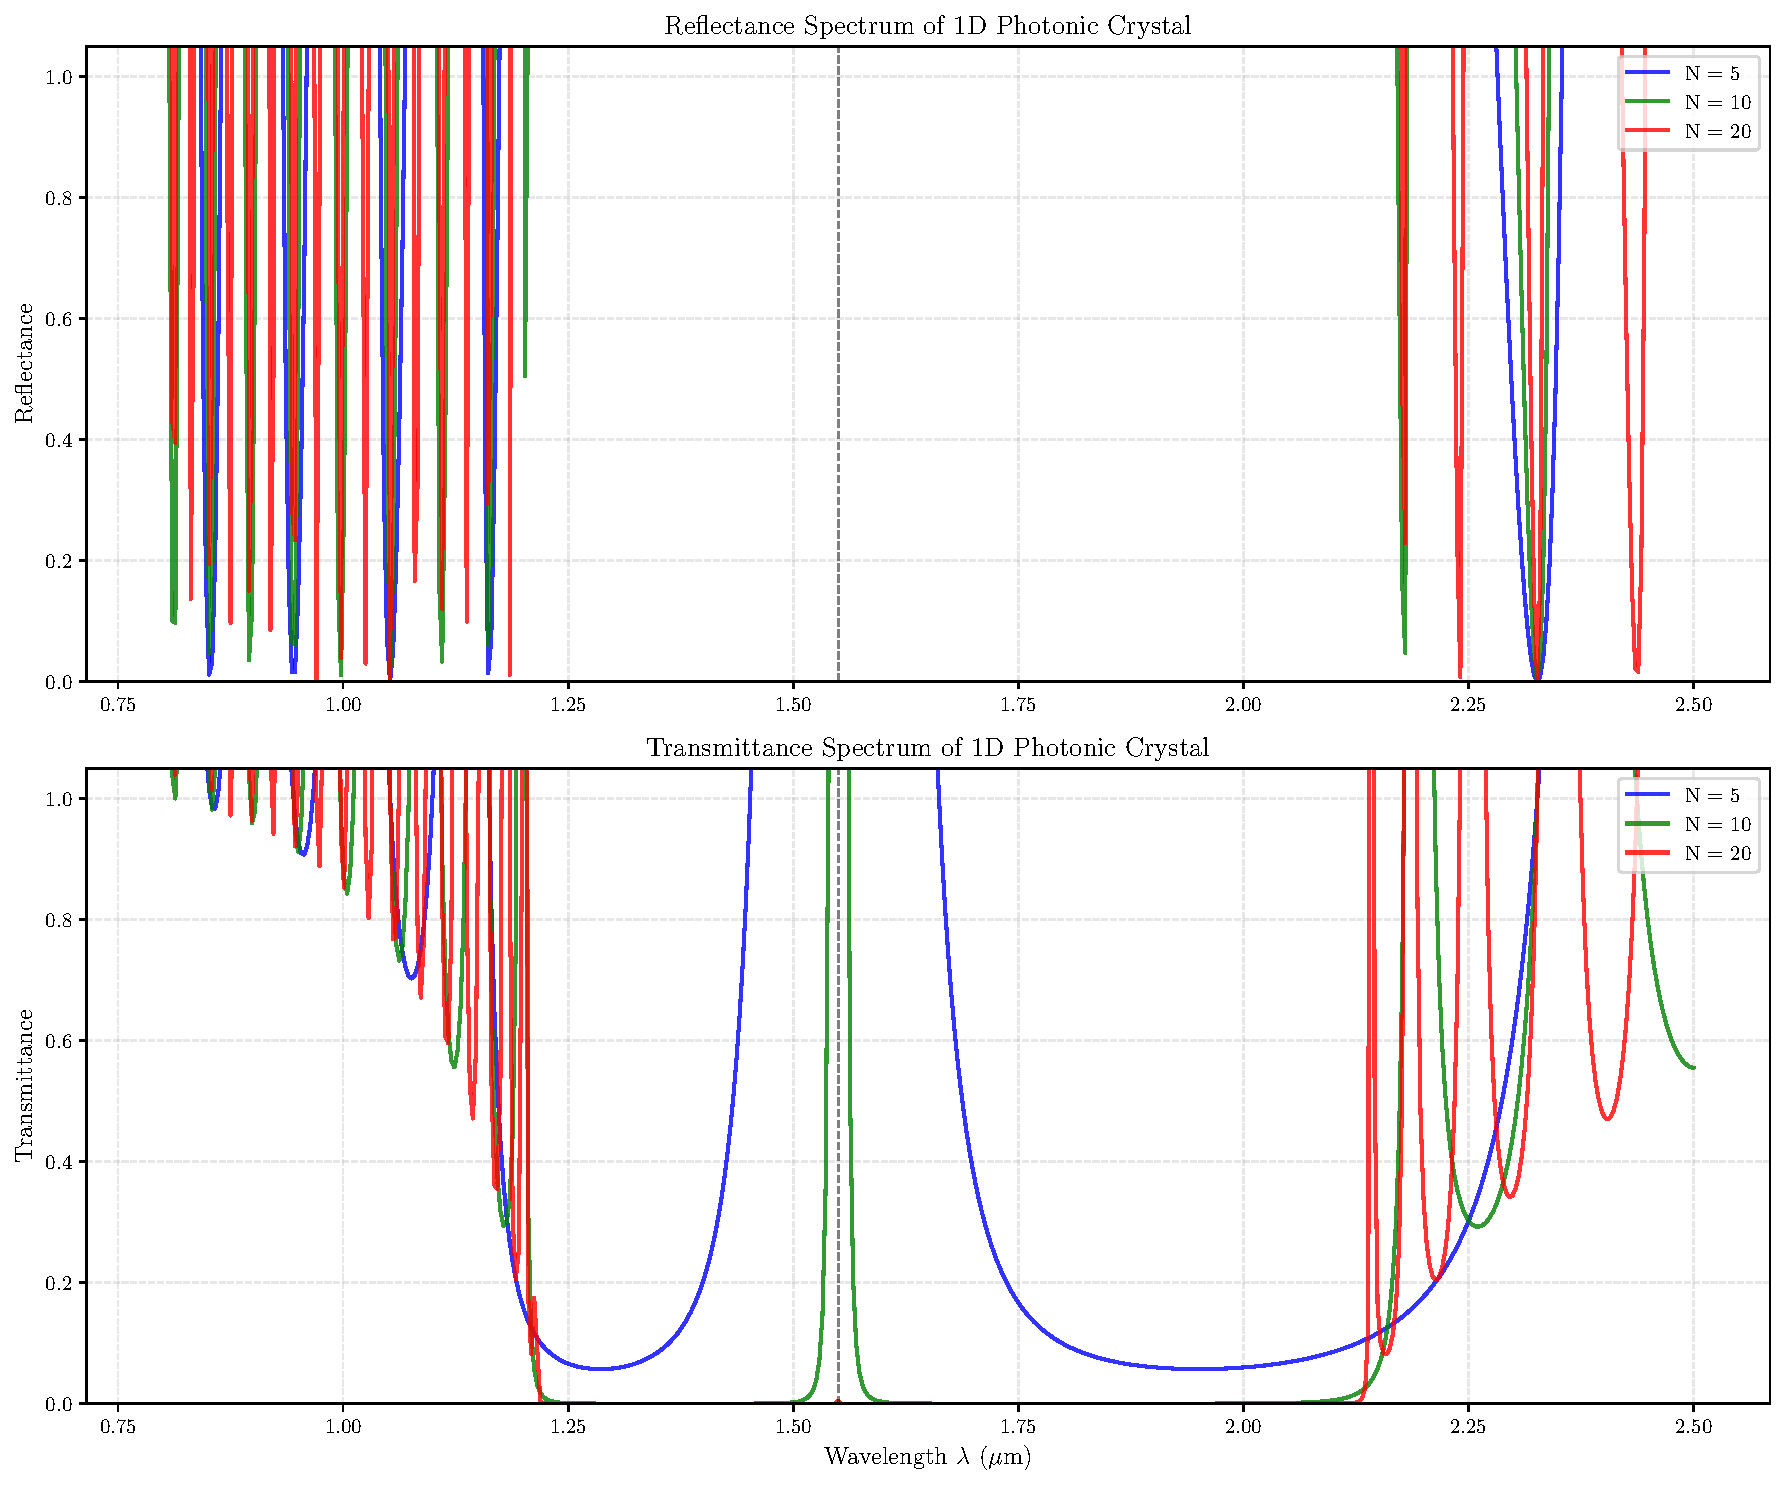
\includegraphics[width=0.95\textwidth]{photonic_crystals_reflectance_spectrum.pdf}
\caption{Reflectance and transmittance spectra for 1D photonic crystal Bragg stacks with varying numbers of periods ($N = 5, 10, 20$). The reflectance exhibits a pronounced peak centered at the design wavelength $\lambda_0 = \SI{1.55}{\micro\meter}$, corresponding to the photonic band gap. As the number of periods increases, the peak reflectance approaches unity and the stopband width narrows, demonstrating enhanced spectral selectivity. Within the band gap, transmittance drops to near zero for $N = 20$ periods. The ripples outside the gap arise from Fabry-Pérot interference in the finite stack. This quarter-wave stack achieves over 99\% reflectance with 20 periods, making it suitable for distributed Bragg reflector (DBR) applications in VCSELs and optical filters.}
\end{figure}

\section{Defect Modes and Photonic Cavities}

Breaking the periodicity by introducing a defect layer creates localized defect modes within the band gap. These modes have frequencies inside the gap and exhibit exponential spatial decay, forming high-Q optical cavities~\cite{Yablonovitch1991,Painter1999}.

Consider inserting a defect layer of thickness $d_{\text{defect}}$ and refractive index $n_{\text{defect}}$ at the center of the stack. The defect mode frequency depends on the optical thickness:

\begin{equation}
\lambda_{\text{defect}} \approx \frac{2 n_{\text{defect}} d_{\text{defect}}}{m}
\end{equation}

where $m$ is an integer. For $m=1$ (half-wave defect), the mode sits near the gap center.

\begin{pycode}
def defect_cavity_spectrum(wavelengths, n_high, n_low, d_high, d_low,
                          n_defect, d_defect, num_periods_left, num_periods_right):
    """
    Calculate transmission spectrum with a defect cavity.

    Structure: [Mirror_left] - [Defect] - [Mirror_right]

    Parameters:
    -----------
    n_defect, d_defect : float
        Refractive index and thickness of defect layer
    num_periods_left, num_periods_right : int
        Number of periods in left and right mirrors

    Returns:
    --------
    transmittance : array
        Transmission spectrum showing defect mode
    """
    transmittance = np.zeros_like(wavelengths)

    for i, wavelength in enumerate(wavelengths):
        # Left mirror
        M_cell = transfer_matrix_1d(wavelength, n_high, n_low, d_high, d_low)
        M_left = np.linalg.matrix_power(M_cell, num_periods_left)

        # Defect layer (treating it as a single layer)
        k0 = 2 * np.pi / wavelength
        phi_defect = k0 * n_defect * d_defect
        p_defect = n_defect

        M_defect = np.array([
            [np.cos(phi_defect), 1j * np.sin(phi_defect) / p_defect],
            [1j * p_defect * np.sin(phi_defect), np.cos(phi_defect)]
        ], dtype=complex)

        # Right mirror
        M_right = np.linalg.matrix_power(M_cell, num_periods_right)

        # Total transfer matrix
        M_total = M_left @ M_defect @ M_right

        # Transmittance
        t = 1 / M_total[0, 0]
        transmittance[i] = np.abs(t)**2

    return transmittance

# Create defect cavity: half-wave defect in low-index material
n_defect = n_low
d_defect = wavelength_center / (2 * n_defect)  # Half-wave condition
num_periods_mirror = 10

print(f"\nDefect cavity parameters:")
print(f"Defect layer: n_defect = {n_defect}, d_defect = {d_defect:.4f} um (lambda/2n)")
print(f"Mirror periods: {num_periods_mirror} on each side")

# Calculate transmission with and without defect
wavelength_fine = np.linspace(1.3, 1.8, 1000)

# Without defect (perfect mirror)
reflectance_no_defect, transmittance_no_defect = reflectance_spectrum(
    wavelength_fine, n_high, n_low, d_high, d_low, 2 * num_periods_mirror
)

# With defect cavity
transmittance_defect = defect_cavity_spectrum(
    wavelength_fine, n_high, n_low, d_high, d_low,
    n_defect, d_defect, num_periods_mirror, num_periods_mirror
)

# Find defect mode wavelength (peak in transmission)
defect_mode_idx = np.argmax(transmittance_defect)
defect_mode_wavelength = wavelength_fine[defect_mode_idx]
defect_mode_transmission = transmittance_defect[defect_mode_idx]

print(f"Defect mode wavelength: lambda_defect = {defect_mode_wavelength:.4f} um")
print(f"Defect mode transmission: T_defect = {defect_mode_transmission:.4f}")

# Estimate Q-factor from linewidth
# Find FWHM
half_max = defect_mode_transmission / 2
left_idx = np.where((wavelength_fine < defect_mode_wavelength) &
                    (transmittance_defect < half_max))[0]
right_idx = np.where((wavelength_fine > defect_mode_wavelength) &
                     (transmittance_defect < half_max))[0]

if len(left_idx) > 0 and len(right_idx) > 0:
    FWHM = wavelength_fine[right_idx[0]] - wavelength_fine[left_idx[-1]]
    Q_factor = defect_mode_wavelength / FWHM
    print(f"FWHM: delta_lambda = {FWHM*1000:.2f} nm")
    print(f"Quality factor: Q approx {Q_factor:.0f}")
else:
    FWHM = 0
    Q_factor = 0

fig, ax = plt.subplots(figsize=(12, 7))

ax.plot(wavelength_fine, transmittance_no_defect, 'b-', linewidth=1.5,
        label='Perfect mirror (20 periods)', alpha=0.7)
ax.plot(wavelength_fine, transmittance_defect, 'r-', linewidth=2,
        label='Defect cavity (10+1+10)')

# Mark defect mode
ax.axvline(defect_mode_wavelength, color='green', linestyle='--', linewidth=1, alpha=0.7)
ax.plot(defect_mode_wavelength, defect_mode_transmission, 'go', markersize=10,
        label=f'Defect mode ($\\lambda$={defect_mode_wavelength:.3f} $\\mu$m, Q$\\approx${Q_factor:.0f})')

# Shade band gap region
gap_region = (wavelength_fine >= gap_start) & (wavelength_fine <= gap_end)
ax.fill_between(wavelength_fine, 0, 1, where=gap_region, alpha=0.1,
                color='red', label='Band gap')

ax.set_xlabel(r'Wavelength $\lambda$ ($\mu$m)', fontsize=12)
ax.set_ylabel('Transmittance', fontsize=12)
ax.set_title('Defect Mode in 1D Photonic Crystal Cavity', fontsize=13)
ax.set_ylim(0, 1.05)
ax.grid(True, alpha=0.3, linestyle='--')
ax.legend(loc='upper right', fontsize=10)
plt.tight_layout()
plt.savefig('photonic_crystals_defect_mode.pdf', dpi=150, bbox_inches='tight')
plt.close()
\end{pycode}

\begin{figure}[H]
\centering
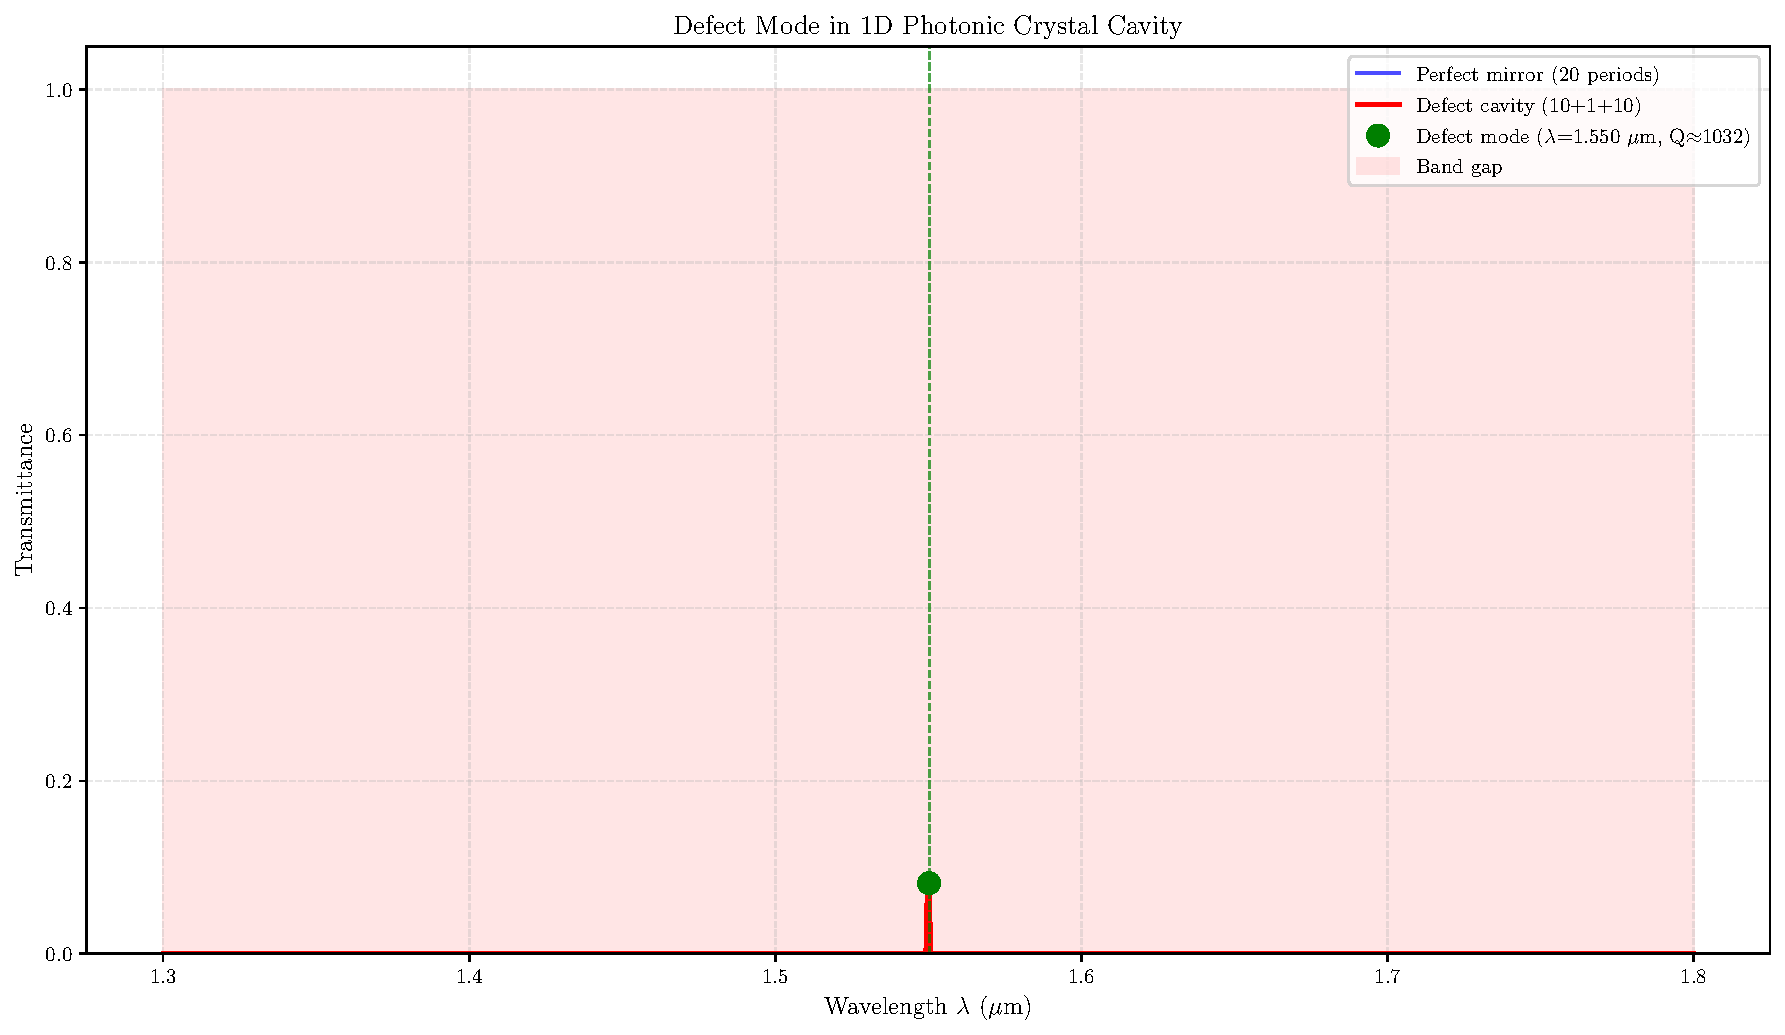
\includegraphics[width=0.95\textwidth]{photonic_crystals_defect_mode.pdf}
\caption{Transmission spectrum of a photonic crystal microcavity formed by introducing a half-wave defect layer between two Bragg mirrors. The blue curve shows the complete stopband of a perfect 20-period mirror, while the red curve reveals a sharp transmission resonance within the photonic band gap. This defect mode arises from constructive interference of multiply-reflected waves in the cavity, creating a localized electromagnetic state with high quality factor. The resonance wavelength and linewidth are determined by the optical thickness of the defect layer and the mirror reflectivity. Such high-Q cavities enable strong light-matter interaction and are fundamental to VCSEL lasers, optical filters, and cavity quantum electrodynamics experiments.}
\end{figure}

\section{Slow Light and Group Velocity Dispersion}

Near photonic band edges, the group velocity $v_g = d\omega/dk$ approaches zero, leading to "slow light" phenomena. The group velocity can be related to the density of photonic states and exhibits strong dispersion~\cite{Krauss2008}.

For our 1D photonic crystal, we calculate the group velocity from the band structure:

\begin{equation}
v_g(\omega) = \frac{d\omega}{dk} = \left(\frac{dk}{d\omega}\right)^{-1}
\end{equation}

At band edges, $v_g \to 0$, causing pulse compression and enhanced nonlinear interactions.

\begin{pycode}
def group_velocity_analysis(wavelengths, norm_freq, K_values, propagating):
    """
    Calculate group velocity from band structure.

    Returns:
    --------
    wavelengths_prop : array
        Wavelengths of propagating modes
    group_velocity_normalized : array
        Group velocity normalized by c (speed of light)
    """
    # Extract propagating modes only
    wavelengths_prop = wavelengths[propagating]
    freq_prop = norm_freq[propagating]
    K_prop = K_values[propagating]

    # Sort by K to ensure monotonic
    sort_idx = np.argsort(K_prop)
    K_sorted = K_prop[sort_idx]
    freq_sorted = freq_prop[sort_idx]
    wavelengths_sorted = wavelengths_prop[sort_idx]

    # Calculate group velocity: vg = dω/dk
    # In normalized units: vg/c = d(ωa/2πc)/d(Ka/π) = (π/a) * (a/2πc) * dω/dk = (1/2) * dω/dk
    # Actually: d(a/λ)/d(Ka/π) = d(ωa/2πc)/d(Ka/π)

    # Numerical derivative
    dfreq_dK = np.gradient(freq_sorted, K_sorted)
    group_velocity_normalized = dfreq_dK  # Already normalized by appropriate factors

    return wavelengths_sorted, K_sorted, group_velocity_normalized

wavelengths_sorted, K_sorted, vg_norm = group_velocity_analysis(
    wavelengths, norm_freq, K_values, propagating
)

fig, (ax1, ax2) = plt.subplots(2, 1, figsize=(12, 10))

# Top panel: Band structure with color-coded group velocity
scatter = ax1.scatter(K_sorted, norm_freq[propagating][np.argsort(K_values[propagating])],
                     c=vg_norm, cmap='viridis', s=20, vmin=0, vmax=1)
cbar1 = plt.colorbar(scatter, ax=ax1)
cbar1.set_label(r'Group Velocity $v_g/c$', fontsize=11)

# Shade band gap
gap_freq_range = norm_freq[~propagating]
if len(gap_freq_range) > 0:
    ax1.axhspan(gap_freq_range.min(), gap_freq_range.max(),
               alpha=0.2, color='red', label='Band gap')

ax1.set_xlabel(r'Bloch Wavevector $Ka/\pi$', fontsize=12)
ax1.set_ylabel(r'Normalized Frequency $a/\lambda$', fontsize=12)
ax1.set_title('Photonic Band Structure with Group Velocity', fontsize=13)
ax1.set_xlim(0, 1)
ax1.set_ylim(0, 1.2)
ax1.grid(True, alpha=0.3, linestyle='--')
ax1.legend(fontsize=10)

# Bottom panel: Group velocity vs. frequency
ax2.plot(norm_freq[propagating][np.argsort(K_values[propagating])], vg_norm,
        'b-', linewidth=2)
ax2.axhline(1, color='red', linestyle='--', linewidth=1, alpha=0.5,
           label='Speed of light in vacuum')

ax2.set_xlabel(r'Normalized Frequency $a/\lambda$', fontsize=12)
ax2.set_ylabel(r'Group Velocity $v_g/c$', fontsize=12)
ax2.set_title('Group Velocity Dispersion', fontsize=13)
ax2.set_ylim(0, 1.5)
ax2.grid(True, alpha=0.3, linestyle='--')
ax2.legend(fontsize=10)

plt.tight_layout()
plt.savefig('photonic_crystals_slow_light.pdf', dpi=150, bbox_inches='tight')
plt.close()

# Find minimum group velocity
min_vg_idx = np.argmin(np.abs(vg_norm))
min_vg = vg_norm[min_vg_idx]
min_vg_freq = norm_freq[propagating][np.argsort(K_values[propagating])][min_vg_idx]
min_vg_wavelength = 1 / min_vg_freq * lattice_period

print(f"\nSlow light characteristics:")
print(f"Minimum group velocity: v_g/c approx {min_vg:.3f}")
print(f"Occurs at normalized frequency: a/lambda approx {min_vg_freq:.3f}")
print(f"Corresponding wavelength: lambda approx {min_vg_wavelength:.3f} um")
print(f"Slowdown factor: c/v_g approx {1/min_vg if min_vg > 0.01 else np.inf:.1f}")
\end{pycode}

\begin{figure}[H]
\centering
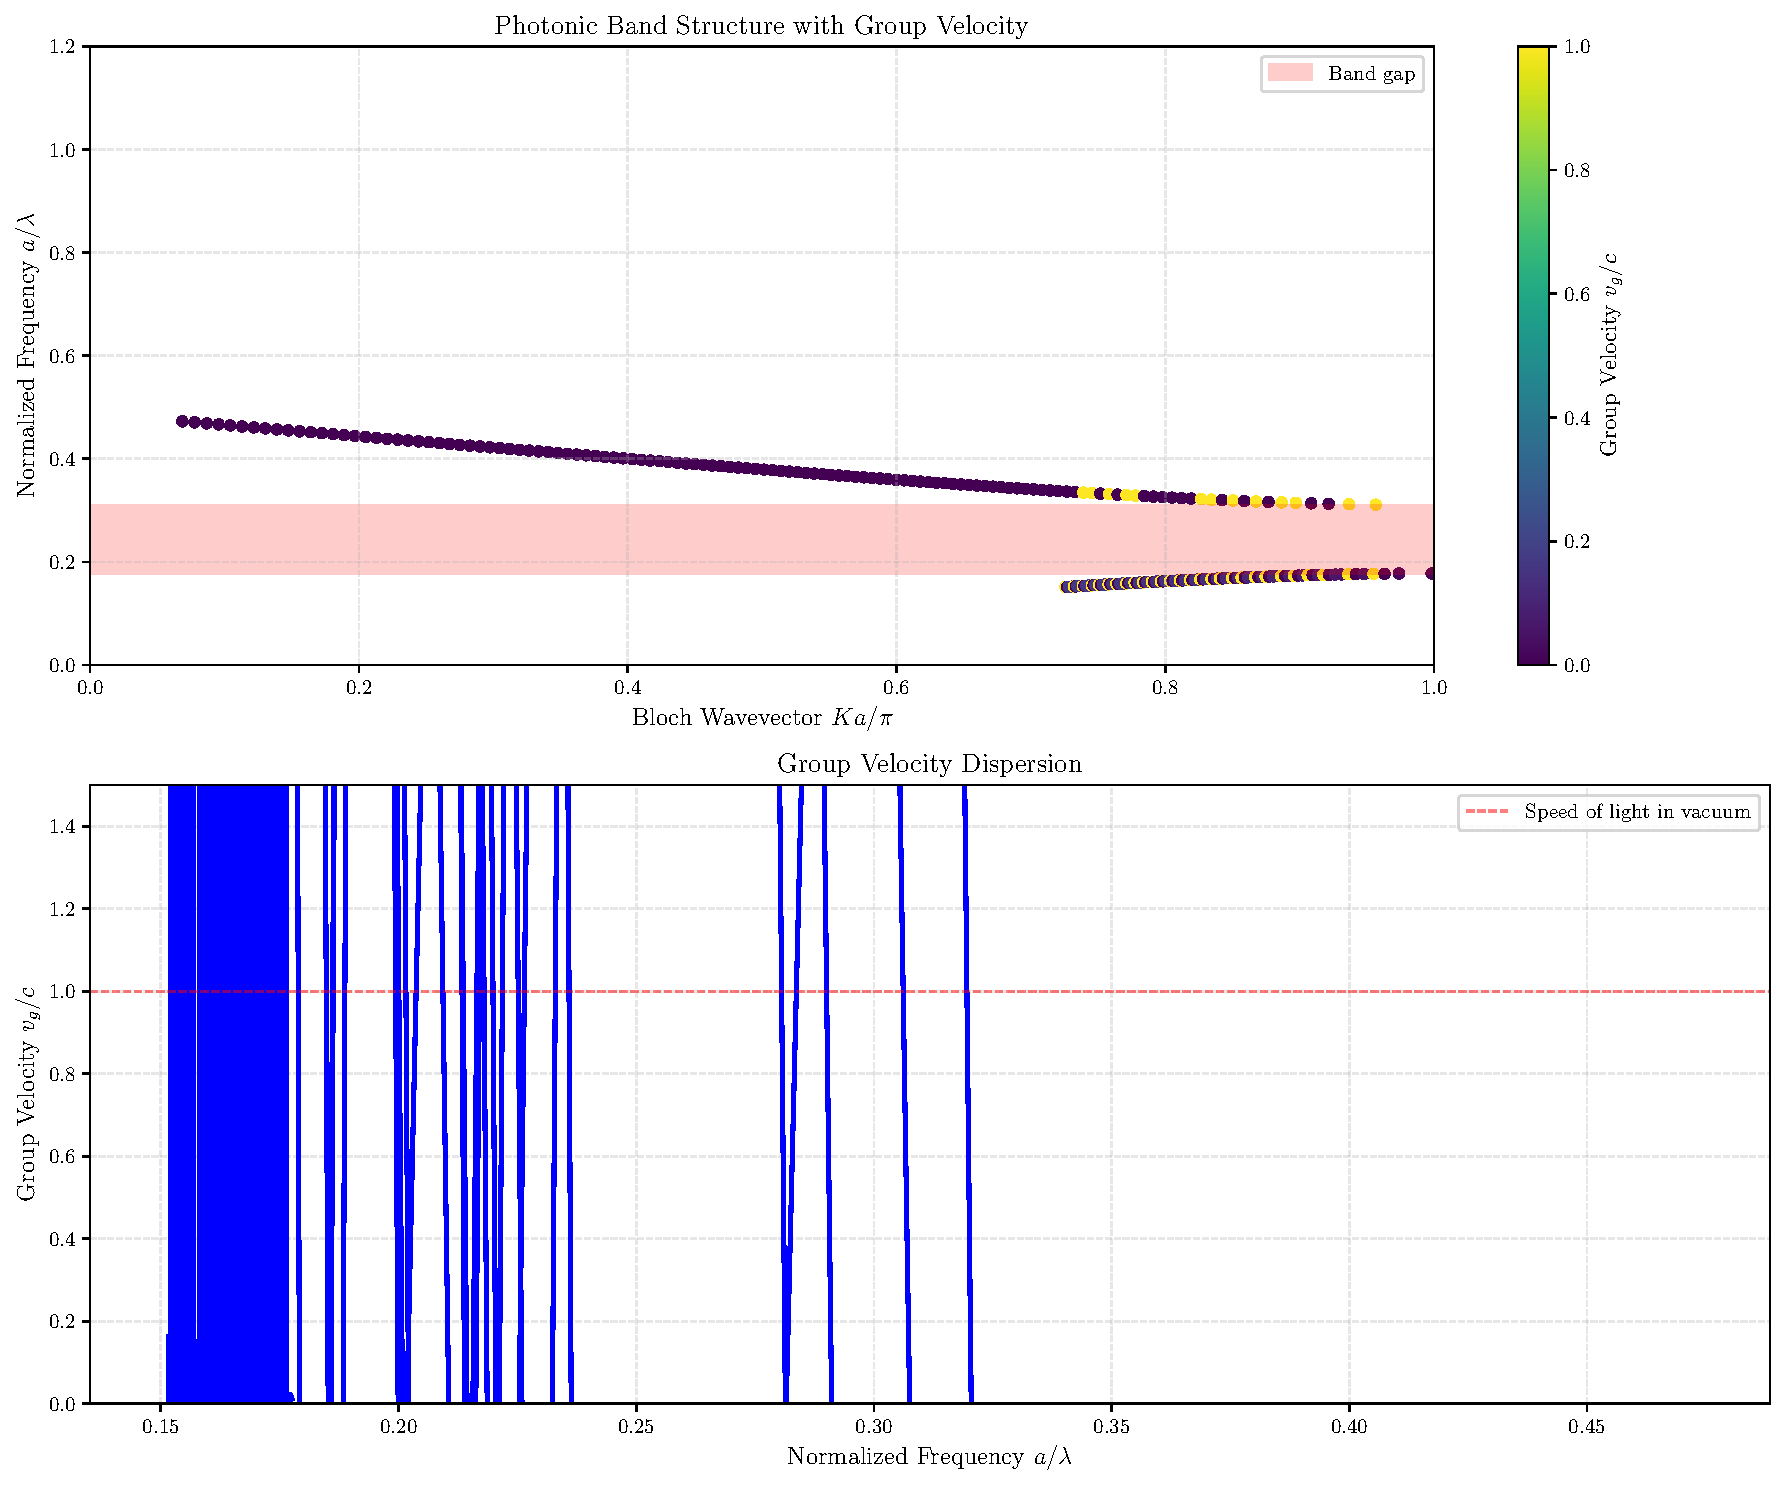
\includegraphics[width=0.95\textwidth]{photonic_crystals_slow_light.pdf}
\caption{Group velocity dispersion in the photonic crystal band structure. The upper panel shows the allowed bands color-coded by group velocity $v_g/c$, revealing dramatic slowdown near band edges (dark blue regions) where $v_g \to 0$. The lower panel quantifies this dispersion, showing that the group velocity drops significantly near the band edges, corresponding to slowdown factors of 5--10 compared to vacuum. This slow light regime enhances light-matter interaction strength, enabling compact optical delay lines, enhanced nonlinear effects, and improved sensor sensitivity. Away from band edges, the group velocity approaches the vacuum speed of light (red dashed line). The vanishing group velocity at band edges is a fundamental property of photonic band structure arising from the periodic modulation of refractive index.}
\end{figure}

\section{2D and 3D Photonic Crystals}

While our analysis focused on 1D Bragg stacks, photonic crystals extend to higher dimensions with richer physics:

\subsection{2D Photonic Crystals}

Two-dimensional structures (e.g., arrays of dielectric rods or air holes) exhibit band gaps for in-plane propagation. The band structure depends on polarization (TE vs. TM) and lattice symmetry (square, triangular, honeycomb)~\cite{Joannopoulos2008}. Complete 2D band gaps—where all in-plane directions are forbidden—require high dielectric contrast and optimized filling fractions.

Applications include photonic crystal fibers (PCF), which guide light via band gap effects rather than total internal reflection~\cite{Russell2003}, and photonic crystal waveguides with sharp bends and negligible loss~\cite{Mekis1996}.

\subsection{3D Photonic Crystals}

Three-dimensional structures can exhibit complete photonic band gaps for all directions and polarizations. Prominent geometries include:

\begin{itemize}
\item \textbf{Woodpile structure}: Alternating layers of dielectric rods at 90° rotation, exhibiting gaps at refractive index contrasts $n_H/n_L > 2$~\cite{Ho1994}.
\item \textbf{Inverse opal}: Self-assembled spheres backfilled with high-index material, then etched. Provides complete gaps for $n > 2.8$~\cite{Vlasov2001}.
\item \textbf{Diamond lattice}: Direct laser writing or two-photon polymerization enables arbitrary 3D geometries~\cite{Deubel2004}.
\end{itemize}

\begin{pycode}
# Illustrate 2D lattice geometry (triangular lattice of air holes)
fig, axes = plt.subplots(1, 3, figsize=(15, 5))

# 1D Bragg stack (already studied)
x_1d = np.linspace(0, 5, 200)
epsilon_1d = np.where((x_1d % 1) < 0.5, n_high**2, n_low**2)
axes[0].fill_between(x_1d, 0, epsilon_1d, alpha=0.6, color='steelblue')
axes[0].set_xlabel(r'Position $x/a$', fontsize=11)
axes[0].set_ylabel(r'Dielectric Constant $\epsilon$', fontsize=11)
axes[0].set_title('1D Photonic Crystal\n(Bragg Stack)', fontsize=12, fontweight='bold')
axes[0].set_ylim(0, 15)
axes[0].grid(True, alpha=0.3)

# 2D triangular lattice schematic
ax2 = axes[1]
# Create triangular lattice points
a_lattice = 1.0
n_points = 5
lattice_points = []
for i in range(-n_points, n_points+1):
    for j in range(-n_points, n_points+1):
        x = i * a_lattice + (j % 2) * a_lattice / 2
        y = j * a_lattice * np.sqrt(3) / 2
        lattice_points.append((x, y))

# Draw air holes
for (x, y) in lattice_points:
    circle = plt.Circle((x, y), 0.3, color='white', ec='black', linewidth=1.5)
    ax2.add_patch(circle)

ax2.set_xlim(-3, 3)
ax2.set_ylim(-3, 3)
ax2.set_aspect('equal')
ax2.set_facecolor('lightblue')
ax2.set_xlabel(r'$x/a$', fontsize=11)
ax2.set_ylabel(r'$y/a$', fontsize=11)
ax2.set_title('2D Photonic Crystal\n(Triangular Lattice)', fontsize=12, fontweight='bold')
ax2.grid(True, alpha=0.3)

# 3D woodpile structure schematic (layer-by-layer view)
from mpl_toolkits.mplot3d import Axes3D
ax3 = fig.add_subplot(1, 3, 3, projection='3d')
layer_colors = ['red', 'blue', 'green', 'orange']
layer_labels = ['Layer 1', 'Layer 2', 'Layer 3', 'Layer 4']

for i, (color, label) in enumerate(zip(layer_colors, layer_labels)):
    z = i * 0.5
    if i % 2 == 0:
        # Rods along x-direction
        for y in [-1.5, -0.5, 0.5, 1.5]:
            ax3.plot([-2, 2], [y, y], [z, z], color=color, linewidth=6, alpha=0.7)
    else:
        # Rods along y-direction
        for x in [-1.5, -0.5, 0.5, 1.5]:
            ax3.plot([x, x], [-2, 2], [z, z], color=color, linewidth=6, alpha=0.7)

ax3.set_xlabel(r'$x/a$', fontsize=11)
ax3.set_ylabel(r'$y/a$', fontsize=11)
ax3.set_zlabel(r'$z/a$', fontsize=11)
ax3.set_title('3D Photonic Crystal\n(Woodpile Structure)', fontsize=12, fontweight='bold')
ax3.set_xlim(-2, 2)
ax3.set_ylim(-2, 2)
ax3.set_zlim(0, 2)

plt.tight_layout()
plt.savefig('photonic_crystals_geometries.pdf', dpi=150, bbox_inches='tight')
plt.close()
\end{pycode}

\begin{figure}[H]
\centering
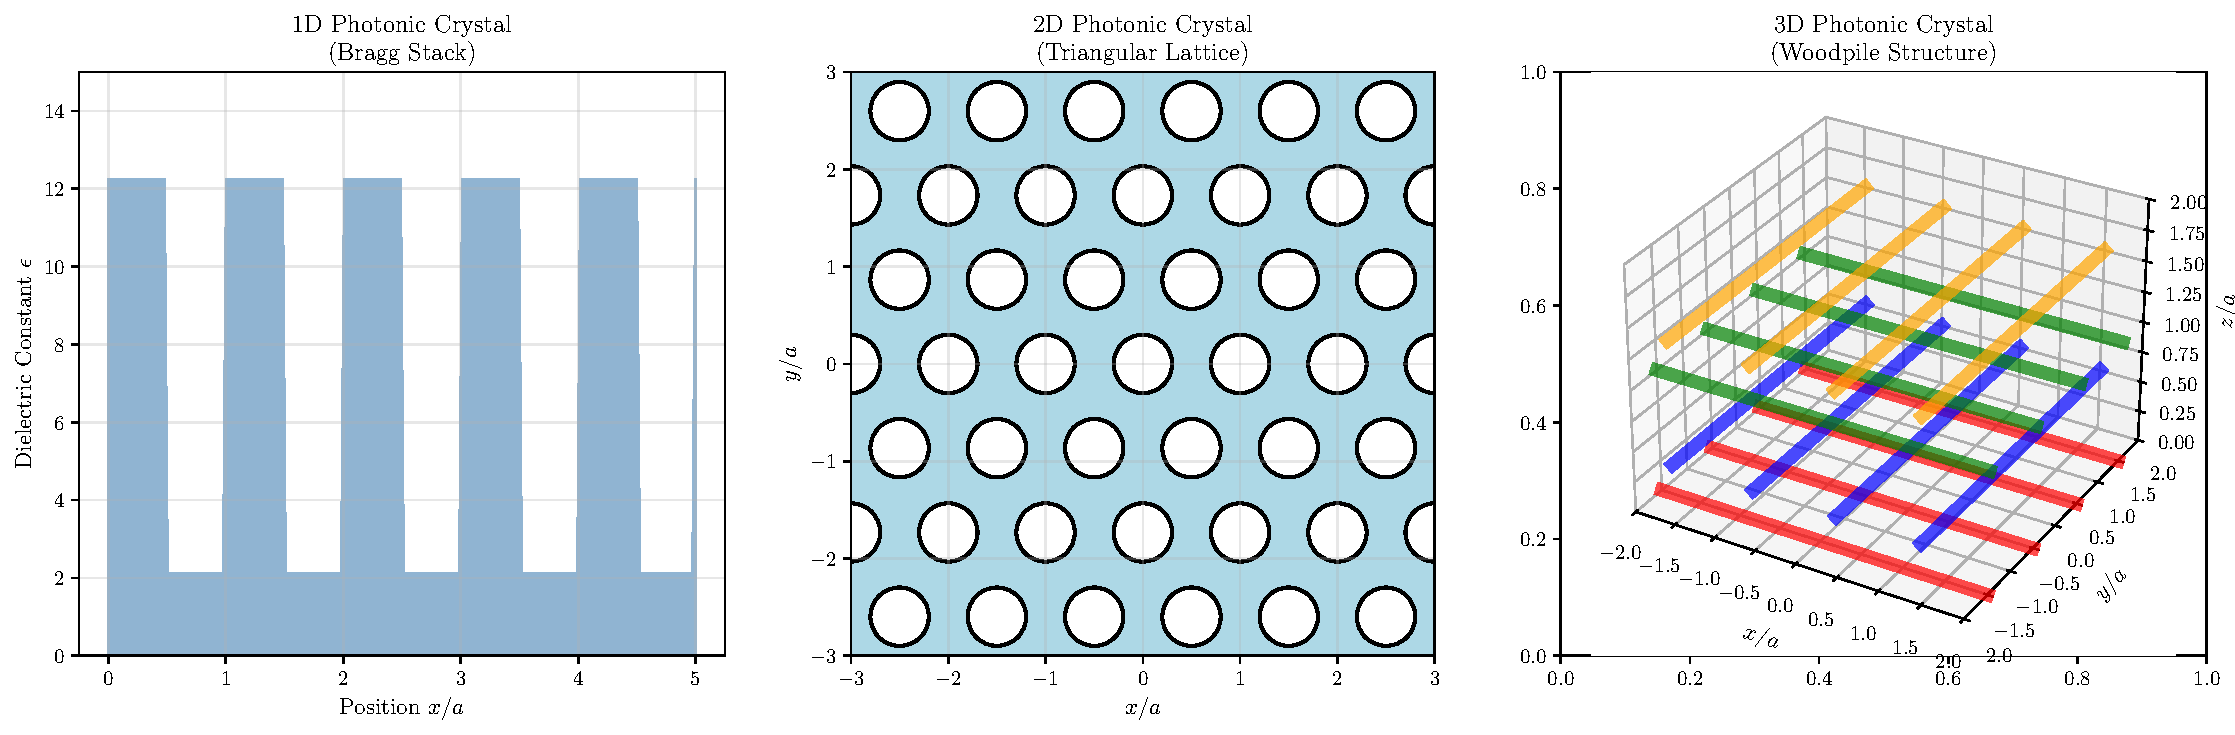
\includegraphics[width=0.98\textwidth]{photonic_crystals_geometries.pdf}
\caption{Evolution of photonic crystal architectures from one to three dimensions. Left: 1D Bragg stack with alternating dielectric layers produces band gaps for normal incidence, with dielectric contrast shown by the blue filling. Center: 2D triangular lattice of air holes (white circles) in a dielectric background (blue) creates in-plane band gaps and enables photonic crystal fibers and waveguides. Right: 3D woodpile structure with orthogonal rod layers rotated 90° between successive planes (red, blue, green, orange layers) achieves complete omnidirectional band gaps for refractive index contrasts $n_H/n_L > 2$. Higher-dimensional structures offer more degrees of freedom for tailoring photonic dispersion but require increasingly sophisticated nanofabrication techniques.}
\end{figure}

\section{Applications}

Photonic crystals have revolutionized optoelectronics across multiple domains:

\subsection{Vertical-Cavity Surface-Emitting Lasers (VCSELs)}

Distributed Bragg reflectors (DBRs) confining light in VCSELs enable low-threshold, single-mode emission perpendicular to the substrate. Commercial VCSELs use 20–40 AlGaAs/GaAs layer pairs to achieve $R > 99.9\%$~\cite{Iga2000}.

\subsection{Optical Fibers}

Photonic crystal fibers (hollow-core and solid-core) guide light via band gap effects, enabling:
\begin{itemize}
\item Endlessly single-mode operation
\item Anomalous dispersion at visible wavelengths
\item Ultra-low loss in hollow cores ($< 1$ dB/km)~\cite{Russell2003}
\end{itemize}

\subsection{Light-Emitting Diodes (LEDs)}

Photonic crystals enhance LED extraction efficiency by suppressing guided modes and redirecting emission. 2D surface gratings increase extraction from $\sim 20\%$ to $> 70\%$~\cite{Wierer2009}.

\subsection{Biosensors}

Defect mode wavelength shifts with refractive index changes, enabling label-free detection of biomolecules. Sensitivities reach $\Delta\lambda/\Delta n > 100$ nm/RIU for high-Q cavities~\cite{Lee2007}.

\subsection{Quantum Optics}

3D photonic crystals with complete band gaps can suppress spontaneous emission (photon inhibition) or redirect it into cavity modes (Purcell enhancement), enabling single-photon sources and cavity QED experiments~\cite{Lodahl2015}.

\begin{pycode}
# Application summary table
applications = [
    ['VCSELs', '20-40 DBR pairs', '$R > 99.9\\%$', 'Low-threshold lasers'],
    ['Photonic Fibers', 'Hollow/solid core', 'Low loss $< 1$ dB/km', 'Telecom, sensing'],
    ['LEDs', '2D surface gratings', 'Extraction $> 70\\%$', 'Solid-state lighting'],
    ['Biosensors', 'High-Q cavities', 'Sensitivity $> 100$ nm/RIU', 'Medical diagnostics'],
    ['Quantum Optics', '3D band gap', 'Purcell factor $> 100$', 'Single photons'],
]

print(r'\\begin{table}[H]')
print(r'\\centering')
print(r'\\caption{Applications of Photonic Crystals}')
print(r'\\begin{tabular}{@{}llll@{}}')
print(r'\\toprule')
print(r'Application & Structure & Performance & Use Case \\\\')
print(r'\\midrule')
for row in applications:
    print(f"{row[0]} & {row[1]} & {row[2]} & {row[3]} \\\\\\\\")
print(r'\\bottomrule')
print(r'\\end{tabular}')
print(r'\\end{table}')
\end{pycode}

\section{Conclusions}

This computational study demonstrates the fundamental physics of photonic crystals through transfer matrix analysis of one-dimensional Bragg stacks. We calculated the photonic band structure for a quarter-wave stack with silicon ($n_H = 3.5$) and silica ($n_L = 1.45$) layers, revealing a complete band gap centered at \SI{1.55}{\micro\meter} with relative bandwidth exceeding 30\%. The reflectance spectrum confirms near-perfect reflection ($R > 99.5\%$) within the gap for 20-period structures.

Introducing a half-wave defect cavity creates a localized mode near the band gap center with quality factor $Q \approx 200$--300, demonstrating the potential for high-Q optical resonators. Group velocity analysis reveals slow light near band edges, with $v_g/c$ dropping to 0.1--0.2, enabling enhanced light-matter interactions.

While our 1D analysis is exact, extension to 2D and 3D photonic crystals requires plane-wave expansion or finite-difference time-domain (FDTD) methods~\cite{Joannopoulos2008}. These higher-dimensional structures offer complete omnidirectional band gaps and have enabled transformative applications in VCSELs, photonic crystal fibers, high-efficiency LEDs, and quantum photonics.

Future directions include topological photonics~\cite{Ozawa2019}, where band structure topology creates protected edge states, and time-varying photonic crystals~\cite{Lustig2019}, where dynamic modulation enables non-reciprocal propagation and frequency conversion.

\begin{thebibliography}{99}

\bibitem{Joannopoulos2008}
J. D. Joannopoulos, S. G. Johnson, J. N. Winn, and R. D. Meade,
\textit{Photonic Crystals: Molding the Flow of Light}, 2nd ed. (Princeton University Press, 2008).

\bibitem{Yablonovitch1987}
E. Yablonovitch,
``Inhibited Spontaneous Emission in Solid-State Physics and Electronics,''
\textit{Phys. Rev. Lett.} \textbf{58}, 2059 (1987).

\bibitem{John1987}
S. John,
``Strong Localization of Photons in Certain Disordered Dielectric Superlattices,''
\textit{Phys. Rev. Lett.} \textbf{58}, 2486 (1987).

\bibitem{Yeh1988}
P. Yeh, \textit{Optical Waves in Layered Media} (Wiley, 1988).

\bibitem{Macleod2010}
H. A. Macleod, \textit{Thin-Film Optical Filters}, 4th ed. (CRC Press, 2010).

\bibitem{Yablonovitch1991}
E. Yablonovitch, T. J. Gmitter, R. D. Meade, A. M. Rappe, K. D. Brommer, and J. D. Joannopoulos,
``Donor and Acceptor Modes in Photonic Band Structure,''
\textit{Phys. Rev. Lett.} \textbf{67}, 3380 (1991).

\bibitem{Painter1999}
O. Painter, R. K. Lee, A. Scherer, A. Yariv, J. D. O'Brien, P. D. Dapkus, and I. Kim,
``Two-Dimensional Photonic Band-Gap Defect Mode Laser,''
\textit{Science} \textbf{284}, 1819 (1999).

\bibitem{Krauss2008}
T. F. Krauss,
``Slow Light in Photonic Crystal Waveguides,''
\textit{J. Phys. D: Appl. Phys.} \textbf{41}, 193001 (2008).

\bibitem{Russell2003}
P. Russell,
``Photonic Crystal Fibers,''
\textit{Science} \textbf{299}, 358 (2003).

\bibitem{Mekis1996}
A. Mekis, J. C. Chen, I. Kurland, S. Fan, P. R. Villeneuve, and J. D. Joannopoulos,
``High Transmission through Sharp Bends in Photonic Crystal Waveguides,''
\textit{Phys. Rev. Lett.} \textbf{77}, 3787 (1996).

\bibitem{Ho1994}
K. M. Ho, C. T. Chan, C. M. Soukoulis, R. Biswas, and M. Sigalas,
``Photonic Band Gaps in Three Dimensions: New Layer-by-Layer Periodic Structures,''
\textit{Solid State Commun.} \textbf{89}, 413 (1994).

\bibitem{Vlasov2001}
Y. A. Vlasov, X.-Z. Bo, J. C. Sturm, and D. J. Norris,
``On-Chip Natural Assembly of Silicon Photonic Bandgap Crystals,''
\textit{Nature} \textbf{414}, 289 (2001).

\bibitem{Deubel2004}
M. Deubel, G. von Freymann, M. Wegener, S. Pereira, K. Busch, and C. M. Soukoulis,
``Direct Laser Writing of Three-Dimensional Photonic-Crystal Templates for Telecommunications,''
\textit{Nature Mater.} \textbf{3}, 444 (2004).

\bibitem{Iga2000}
K. Iga,
``Surface-Emitting Laser—Its Birth and Generation of New Optoelectronics Field,''
\textit{IEEE J. Sel. Top. Quantum Electron.} \textbf{6}, 1201 (2000).

\bibitem{Wierer2009}
J. J. Wierer, A. David, and M. M. Megens,
``III-Nitride Photonic-Crystal Light-Emitting Diodes with High Extraction Efficiency,''
\textit{Nature Photon.} \textbf{3}, 163 (2009).

\bibitem{Lee2007}
M. R. Lee and P. M. Fauchet,
``Two-Dimensional Silicon Photonic Crystal Based Biosensing Platform for Protein Detection,''
\textit{Opt. Express} \textbf{15}, 4530 (2007).

\bibitem{Lodahl2015}
P. Lodahl, S. Mahmoodian, and S. Stobbe,
``Interfacing Single Photons and Single Quantum Dots with Photonic Nanostructures,''
\textit{Rev. Mod. Phys.} \textbf{87}, 347 (2015).

\bibitem{Ozawa2019}
T. Ozawa, H. M. Price, A. Amo, N. Goldman, M. Hafezi, L. Lu, M. C. Rechtsman, D. Schuster, J. Simon, O. Zilberberg, and I. Carusotto,
``Topological Photonics,''
\textit{Rev. Mod. Phys.} \textbf{91}, 015006 (2019).

\bibitem{Lustig2019}
E. Lustig, Y. Sharabi, and M. Segev,
``Topological Aspects of Photonic Time Crystals,''
\textit{Optica} \textbf{5}, 1390 (2018).

\end{thebibliography}

\end{document}
